\chapter{Analyse de la base de données d’IMPatienT par IA Explicable (xAI)}

La création d'un vocabulaire standard décrivant les observations (termes) faites lors de la biopsie musculaire a permis grâce à \gls{impatient} la numérisation de 89 rapports de biopsie de patients atteints de \gls{mc}. En utilisant \gls{impatient} comme outil pour structurer les comptes rendus de biopsie en texte libre sous forme de données annotées, nous pouvons alors utiliser des méthodes de \gls{ml} traditionnel pour entraîner des modèles prédicatifs. Bien que les méthodes de \gls{ml} traditionnelles soient restreintes à l'analyse de données bien structurée et annotées, elles présentent l'avantage de pouvoir être utilisable même avec une quantité de données faible (ce qui est le cas dans les maladies rares). De plus, ces méthodes présentent une meilleure explicabilité que les méthodes à base de réseau de neurones profonds. L'explicabilité d'un modèle prédictif destiné à l'aide au diagnostic est cruciale pour permettre d'avoir confiance et d'évaluer une suggestion de diagnostic automatique en médecine. Ainsi dans ce chapitre, nous avons voulu comparer les performances de plusieurs modèles de \gls{ml} avec une exploration plus spécifique d'un modèle de \gls{lcs} considérée comme référence parmi les algorithmes explicatifs en entraînant ces modèles sur la base de données d'\gls{impatient}.

\section{Contenu de la base de données}
Les 89 rapports d'histologie ont été numérisés en annotant \textit{via} \gls{impatient} chacun des termes du vocabulaire entre: absence du terme (0), présence (suivant 4 gradations de quantité de 0,25 à 1) ou absence d'information (N/A). Cette procédure a permis d'obtenir une matrice numérique de taille (89x175) où les 175 colonnes représentent les 175 termes du vocabulaire standard. De plus, pour chacun des 89 rapports, un certain nombre de métadonnées ont été enregistrées telles que: l'âge, le numéro de biopsie, le muscle, le diagnostic final, l'identifiant de la biopsie, l'identifiant unique du patient.
\subsection{Analyse statistique exploratoire}
Dans un premier temps, j'ai réalisé une analyse statistique exploratoire de ce jeu de données (figure \ref{fig:impatient_eda} et figure \ref{fig:impatient_eda2}). Ainsi, grâce à \gls{impatient}, nous avons généré plusieurs visualisations dont des histogrammes (fig. \ref{fig:impatient_eda}, des matrices de corrélation (fig. \ref{fig:impatient_eda2}), des tableaux de fréquences et des matrices de confusion pour évaluer la méthode \gls{boqa}. On observe dans notre jeu de données une majorité de patients adultes (49 sur 89). Au niveau des gènes, les gènes TTN, NEB, RYR1 et MYH7 sont les plus souvent responsables de la maladie (40 sur 89). Au niveau des maladies, les \gls{com} et les \gls{nm} sont les plus communes (28 et 25). Ensuite, on remarque un grand groupe de 23 patients sans diagnostic clairement établi et un groupe plus restreint de 10 patients à \gls{cnm}. Le tableau des termes les plus fréquents par diagnostic (accessible en ligne: \url{https://lbgi.fr/~meyer/stat_per_diag.xlsx} et dans l'archive Zenodo) fait ressortir des termes attendus tels qu’une forte fréquence de bâtonnets sombres dans les \gls{nm}, de noyaux centralisés dans les \gls{cnm} et de prédominance de fibre de type 1, de taille inégale des fibres et de cores (cores centraux uniques et cores périphériques) dans les \gls{com}.

\begin{figure}[!ht]
  \centering
  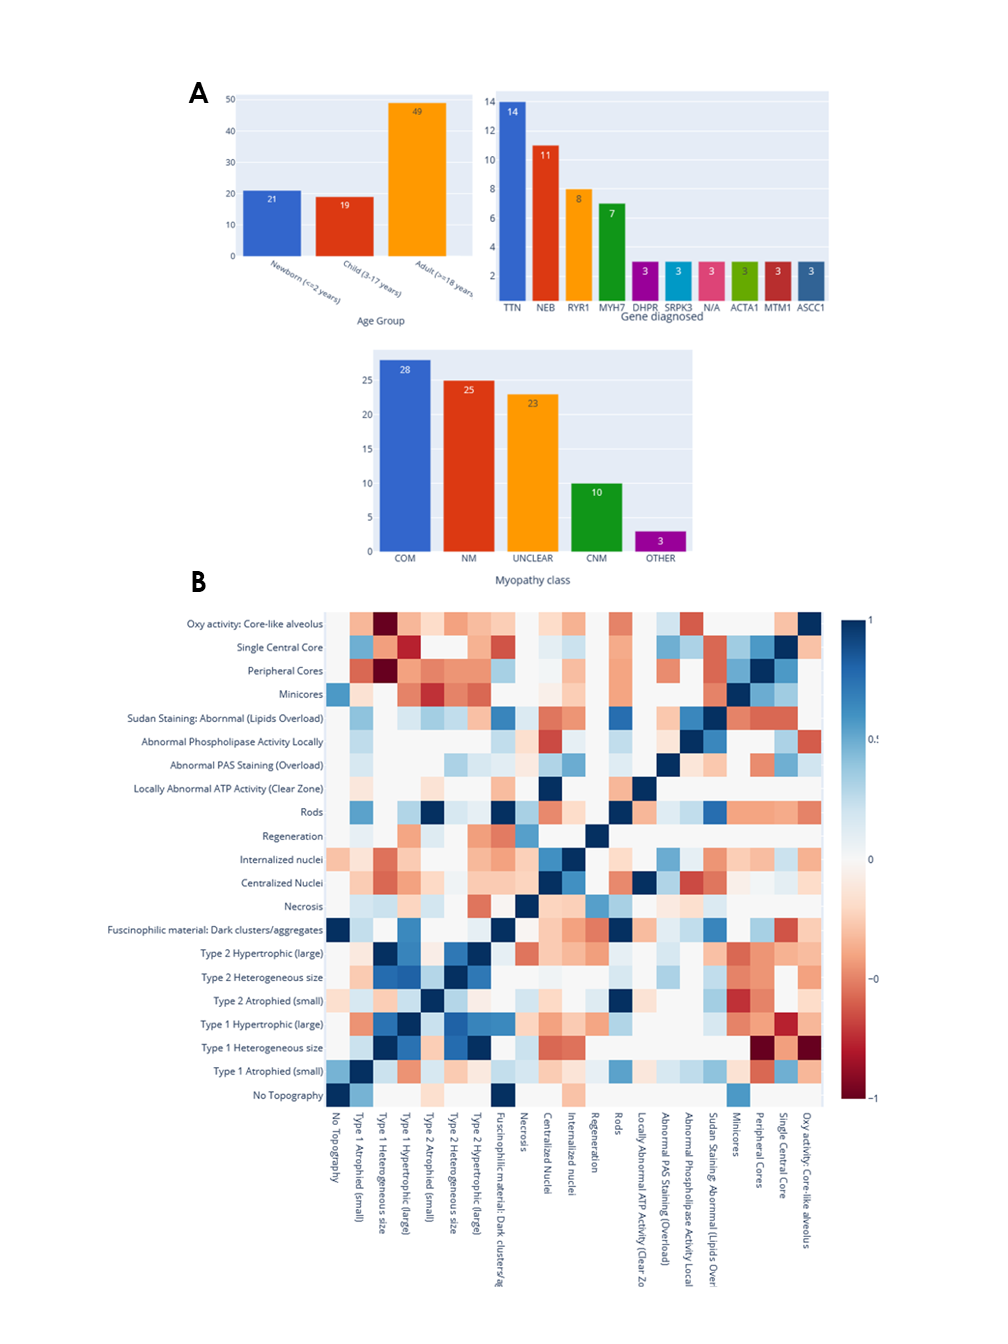
\includegraphics[width=1\textwidth]{figures/impatient_explo.png}
  \caption[Analyse statistique exploratoire IMPatienT (histogrammes)]{\textbf{Analyse statistique exploratoire de la base de données IMPatienT}: Histogrammes de répartition des patients en fonction de leur groupe d'âge, du gène muté responsable de la maladie et de leur classe de myopathie (némaline, core, centronucléaire, autre (OTHER) et pas de diagnostic établi (UNCLEAR).}
  \label{fig:impatient_eda}
\end{figure}
\begin{figure}[!ht]
  \centering
  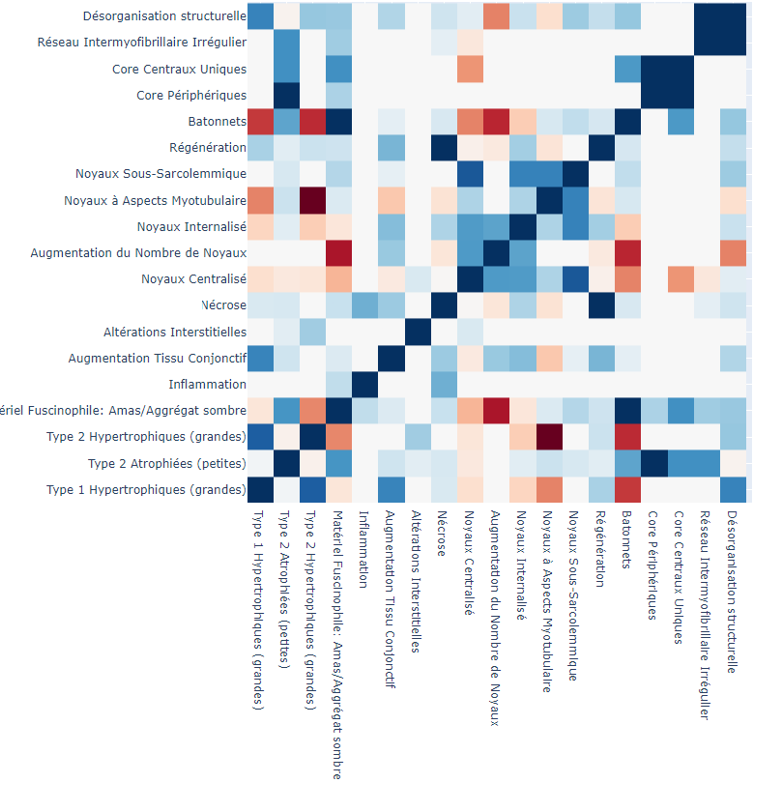
\includegraphics[width=0.8\textwidth]{figures/impatient_explo2.png}
  \caption[Analyse statistique exploratoire IMPatienT (matrice)]{\textbf{Analyse statistique exploratoire de la base de données IMPatienT}: Matrice de corrélation partielle des termes du vocabulaire standard. La couleur rouge indique une corrélation négative (-1), la couleur bleue une corrélation positive (+1). Deux termes avec une corrélation positive sont deux termes qui ont une forte co-occurrence chez les patients.}
  \label{fig:impatient_eda2}
\end{figure}

\section{Pipeline de Machine-Learning Streamline}
Nous avons voulu évaluer s'il était possible de prédire le diagnostic des patients \textit{via} des techniques de classification par algorithmes de \gls{ml} traditionnels. Pour cela, nous avons utilisé et modifié le pipeline Streamline (\cite{urbanowicz_streamline_2023}), développé par \textit{Ryan J. Urbanowicz}, créateur aussi de l'algorithme de classification explicable (de type \gls{lcs}) nommé ExSTraCS 2.0 (\cite{urbanowicz_exstracs_2015}).
Le pipeline Streamline permet d'entraîner, d'optimiser et de comparer 11 algorithmes traditionnels de \gls{ml} sur un même jeu de données. Ce pipeline est développé pour la classification binaire, j'ai donc procédé à des modifications pour le rendre compatible avec des tâches de classification multi-classes (prédiction de diagnostic entre les \gls{nm}, \gls{com} et les \gls{cnm}).
\section{Résultats d'analyse}
L'utilisation de Streamline nous a permis de comparer 11 algorithmes de \gls{ml} pour la classification de données biomédicales (tableau \ref{table:ml_metrics}). Les 11 algorithmes ont montré une exactitude de classification (métrique qui considère le pourcentage de classification correcte au global) se situant entre 0,71 et 0,86. Si l’on regarde les performances pour le coefficient de corrélation de Matthew (la seule métrique de performance prenant en compte l'ensemble de la matrice de confusion) l'écart entre les algorithmes est encore plus faible. Dix des onze algorithmes ont un score \gls{mcc} compris entre 0,72 et 0,79. Au niveau de la courbe ROC (comparaison du taux de vrais positifs par rapport aux faux positifs pour différents seuils), les algorithmes semblent similaires, alors une aire sous la courbe (\textit{area under the curve}, AUC) légèrement en deçà des autres algorithmes pour ExSTraCS et l'arbre de décision (aux alentours de 0.85 contre 0.90 et 0.95 pour les neuf autres, \ref{fig:roc_curve}).
\begin{figure}[!ht]
  \centering
  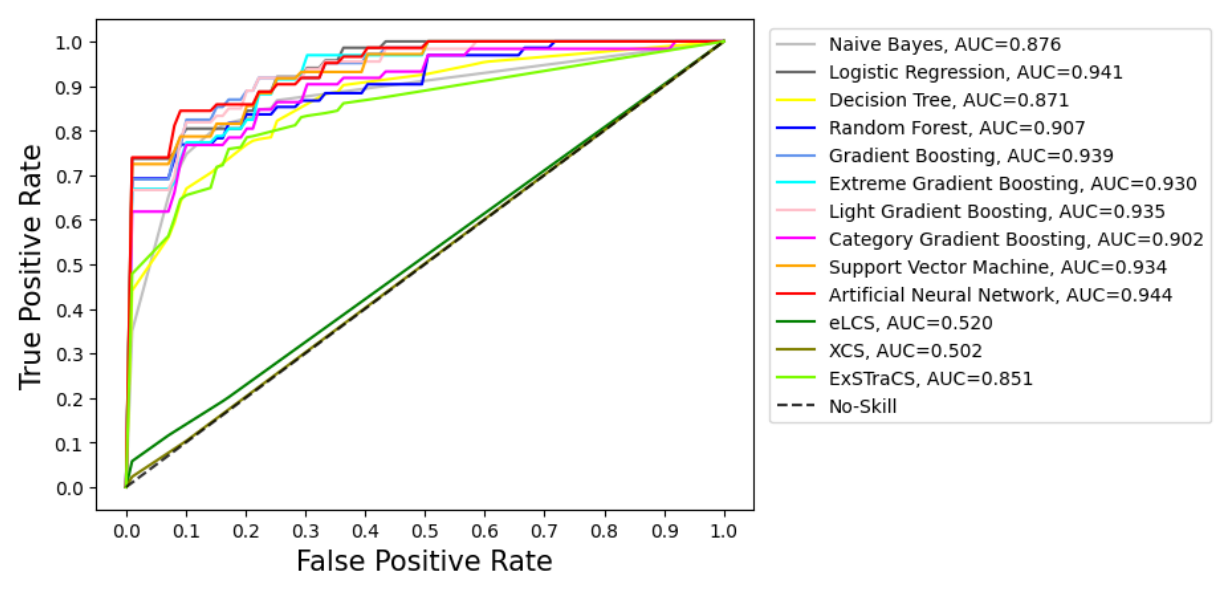
\includegraphics[width=1\textwidth]{figures/roc_streamline.png}
  \caption[Comparaison des courbes ROC]{\textbf{Comparaison des courbes ROC des 11 algorithmes comparés}. La valeur AUC représente l'aire sous la courbe, plus elle est proche de 1 plus le modèle est performant.}
  \label{fig:roc_curve}
\end{figure}
\begin{table}[!ht]
\centering
\begin{tabular}{lcccc}
\hline
Algorithme & Exactitude Équilibrée & Exactitude & Matthew Corr. Coeff. & Spécificité  \\
\hline
Bayesienne Naive & 0.67 & 0.82 & 0.74 & 0.91 \\
Regession Logistique & 0.86 & 0.82 & 0.72 & 0.91 \\
Arbre de décision & 0.72 & 0.72 & 0.74 & 0.86 \\
Forêt Aléatoire & 0.81 & 0.82 & 0.74 & 0.91 \\
Boosting & \textbf{0.89} & 0.85 & 0.78 & 0.92 \\
XGBoost & 0.75 & 0.82 & 0.74 & 0.91 \\
LGBoost & 0.67 & 0.83 & 0.76 & 0.92 \\
CatBoost & 0.67 & 0.82 & 0.73 & 0.91 \\
SVM & \textbf{0.89} & 0.85 & \textbf{0.79} & 0.92 \\
Perceptron & 0.67 & \textbf{0.86} & 0.78 & \textbf{0.93}\\
ExSTraCS & 0.61 & 0.71 & 0.61 & 0.86 \\
\hline
\end{tabular}
\caption[Comparaison des performances des modèles (moyenne sur 10 folds de cross-validation)]{\textbf{Comparaison des performances des modèles (moyenne sur 10 \textit{folds} de cross-validation)}. Les méthodes SVM et Boosting ont obtenu les meilleures performances à travers la majorité des métriques. La méthode LCS ExSTraCS a obtenu des performances 22\% inférieurs aux meilleurs modèles.}
\label{table:ml_metrics}
\end{table}        
Les algorithmes \gls{svm} et \textit{Boosting } se sont révélés être les meilleurs algorithmes en termes d'exactitude équilibrée et de score \gls{mcc}, cependant ces deux modèles ne sont pas des modèles transparents et nécessitent de méthodes \textit{post-hoc} pour interpréter les prédictions (explicabilité). L'algorithme ExSTraCS, qui lui est un modèle totalement transparent et explicable, a obtenu des performances 22\% inférieures au meilleur modèle, avec un score \gls{mcc} de 0,61 et une exactitude de 0,71, ce qui est constamment en dessous des autres algorithmes. Cette performance plus faible peut s'expliquer en partie par les contraintes lors de son entraînement lié à l'explicabilité. En effet, nous avons volontairement restreint le nombre de règles que l'algorithme peut générer pour le rendre plus facilement interprétable et pour pouvoir en extraire les principales règles de classification entre les sous-types de myopathies (voir section \ref{lcs_viz_sec}). Il est intéressant de noter que l'algorithme de classification d'arbre de décision, qui est à la fois simple et par nature explicable, a obtenu des performances dans la moyenne des autres algorithmes, tout en ayant un temps d'entraînement faible de 17 secondes en raison de sa simplicité (tableau \ref{tab:pipeline_times}). À titre de comparaison, le \gls{lcs} ExSTraCS a nécessité un temps d'entraînement de 5min39, et ceci sans phase d'optimisation des hyperparamètres.
\begin{table}[!ht]
    \centering
    \begin{tabular}{lc}
        \toprule
        Algorithme & Temps d'optimisation et d'entraînement (sec) \\
        \midrule
        Bayesienne Naive & 11 \\
        Régression Logistique & 30 \\
        Arbre de décision & 17 \\
        Forêt Aléatoire & 2072 \\
        Boosting & 1887 \\
        XGBoost & 733 \\
        LGBoost & 168 \\
        CatBoost & 4578 \\
        SVM & 22 \\
        Perceptron & 389 \\
        ExSTraCS & 339 \\
        \bottomrule
    \end{tabular}
    \caption[Temps d'optimisation des hyperparamètres et d'entrainement des algorithmes de ML]{\textbf{Temps d'optimisation des hyperparamètres et d'entrainement des algorithmes de ML}. Certains modèles simples comme l'arbre de décision, la régression logistique et le modèle SVM ont un temps d'entrainement et d'optimisation inférieur à 1 minute. Les méthodes complexes comme le Boosting, la forêt aléatoire et le LCS ont des temps d'entrainement et d'optimisation supérieurs à 30 minutes.}
    \label{tab:pipeline_times}
\end{table}
\begin{figure}[!ht]
  \centering
  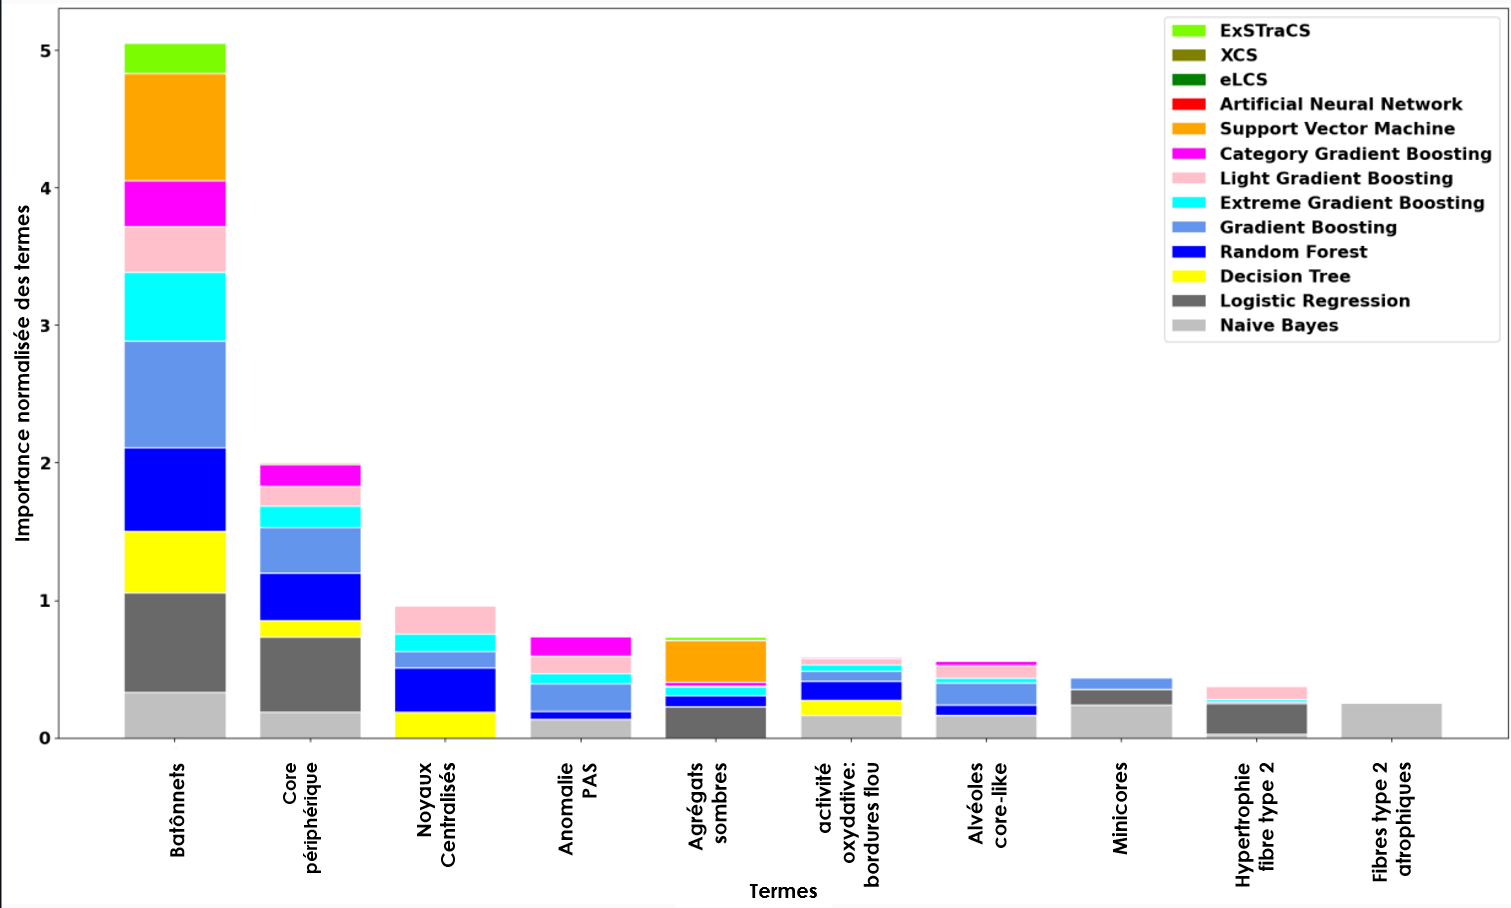
\includegraphics[width=1\textwidth]{figures/feature_importance.png}
  \caption[Histogramme des 10 termes les plus déterminants pour la classification]{\textbf{Histogramme des 10 termes les plus déterminants pour la classification pour chaque algorithme considéré}. Une très grande importance est accordée par tous les algorithmes à la présence de bâtonnets pour faire la différence entre les sous-types de myopathies.}
  \label{fig:feautre_importance}
\end{figure}
L'histogramme montrant les 10 termes les plus importants pour la classification de toutes les classes de \gls{mc} dans l'ensemble des algorithmes (fig. \ref{fig:feautre_importance}) mets en évidence des termes attendus comme la présence de bâtonnets, de cores ou de noyaux centralisés pour différencier \gls{nm}, \gls{com} et \gls{cnm} avec un poids très important pour la présence de bâtonnets. Mais on observe aussi la présence de critères moins attendus, comme la présence d'anomalie au marquage PAS ou l'atrophie des fibres de type 2. De plus on observe aussi que tout les algorithmes n'accordent pas la même importance aux mêmes termes. Par exemple, la présence de fibres de type 2 atrophiques ne semblent importantes que pour la méthodes bayésienne naïve.

La faible taille de notre jeu de données (89 patients), sa grande dimensionalité et hétérogéinité (175 termes) couplé aux faibles différences en termes de performances entre les algorithmes semble restreignantes concernant la comparaison des algorithmes. Sur notre jeu de données, il semblerait que l'utilisation d'algorithmes simples comme l'arbre de décision soit à privilégier pour sa triple efficacité en termes de performances, explicabilité et coût en puissance de calcul. Il est possible que l'utilisation d'un ensemble de données plus important, c’est-à-dire contenant plus de comptes rendus de biopsies, et plus homogènes permettrait une meilleure évaluation des performances de ces algorithmes et, par conséquent, une meilleure compréhension de leurs avantages et inconvénients respectifs dans le contexte de la classification de données biomédicales de manière explicable.

\section{Méthode de visualisation des règles de LCS}\label{lcs_viz_sec}
Bien que notre algorithme de \gls{lcs} présente des performances inférieurs aux autres algorithmes en terme de classification, ils ont l'avantage de produire produisent une liste de règles pour la classification, ce qui rend le processus de prédiction totalement transparent. Cette liste de règles explicites, peut permettre d'utiliser cet algorithme comme extracteur de connaissances à partir de nos données, en découvrant des règles pertintentes de classification qui n'étaient pas connu à priori.

Cependant, une simple liste de règles sous la forme d'un tableau ne permet pas d'extraire des connaissances facilement et rapidement de ces modèles. Nous avons voulu explorer différentes approches pour représenter graphiquement ces règles, afin d'en extraire des connaissances de manière visuelle. Le code écrit pour générer ces visualisations est open source et est disponible dans un répertoire GitHub à l'adresse: \url{https://github.com/lambda-science/PredEx}.

\subsection{Principe général}
Nous avons développé deux approches pour la visualisation des règles produites par l'entrainement de ExSTraCS. Au total, ce sont 42 règles accessibles en ligne à l'adresse \url{https://lbgi.fr/~meyer/lcs_rules.xlsx} ou dans l'archive Zenodo associée qui ont été générées.

La première approche consiste à visualiser les interactions entre les termes dans les rapports, c'est-à-dire leur co-occurrence dans les règles générées. Lorsque deux termes apparaissent dans une même règle définie par un LCS, un lien est tracé entre eux, produisant un diagramme de cordes. Un lien épais entre deux termes indique une co-occurrence importante dans la liste des règles, suggérant une relation étroite entre les termes du vocabulaire standard des biopsies musculaire.
La seconde approche consiste à visualiser les liens entre les termes et les diagnostics. Sur un graphe, chaque nœud circulaire représente un terme, tandis qu'un nœud triangulaire représente un diagnostic. Pour chaque règle, un lien est tracé entre les termes et le diagnostic correspondant. Plus le terme apparait dans des règles liées à un diagnostic, plus le lien sera épais, indiquant une relation forte entre l'observation et la classe de \gls{mc}. Les liens sont colorés en rouge ou vert en fonction de l'absence ou la présence du terme menant à la classe de \gls{mc}, respectivement. Par exemple, si toutes les règles liant le terme "core" aux \gls{nm} stipulent que les cores doivent être absents, alors le lien sera rouge. Si l'observation est liée au diagnostic à la fois en état d'absence et de présence dans des règles différentes, le lien est coloré en jaune, reflétant la complexité de la relation entre l'observation et le diagnostic.
\subsection{Résultats}
La première approche a permis de générer le diagramme de cordes présenté dans la figure \ref{fig:chords}. Cette figure est disponible de manière interactive à l'adresse \url{https://lbgi.fr/~meyer/chord.html} et dans l'archive Zenodo. Sur cette représentation, nous avons filtré les liens pour ne conserver que les liens ayant une valeur supérieure ou égale à 3 (co-occurrence des deux termes dans au moins 3 règles). On observe sur cette figure des interactions complexes et multiples entre les termes. Par exemple, les règles impliquant le terme"Type 1 atrophiées" incluent toujours le terme "sans topographie". De même pour le terme "Type 2 hypertrophiques" et le terme "Activité oxydative: alvéoles core-like", qui apparaissent conjointement dans 4 règles différentes. \clearpage
\begin{figure}[H]
  \centering
  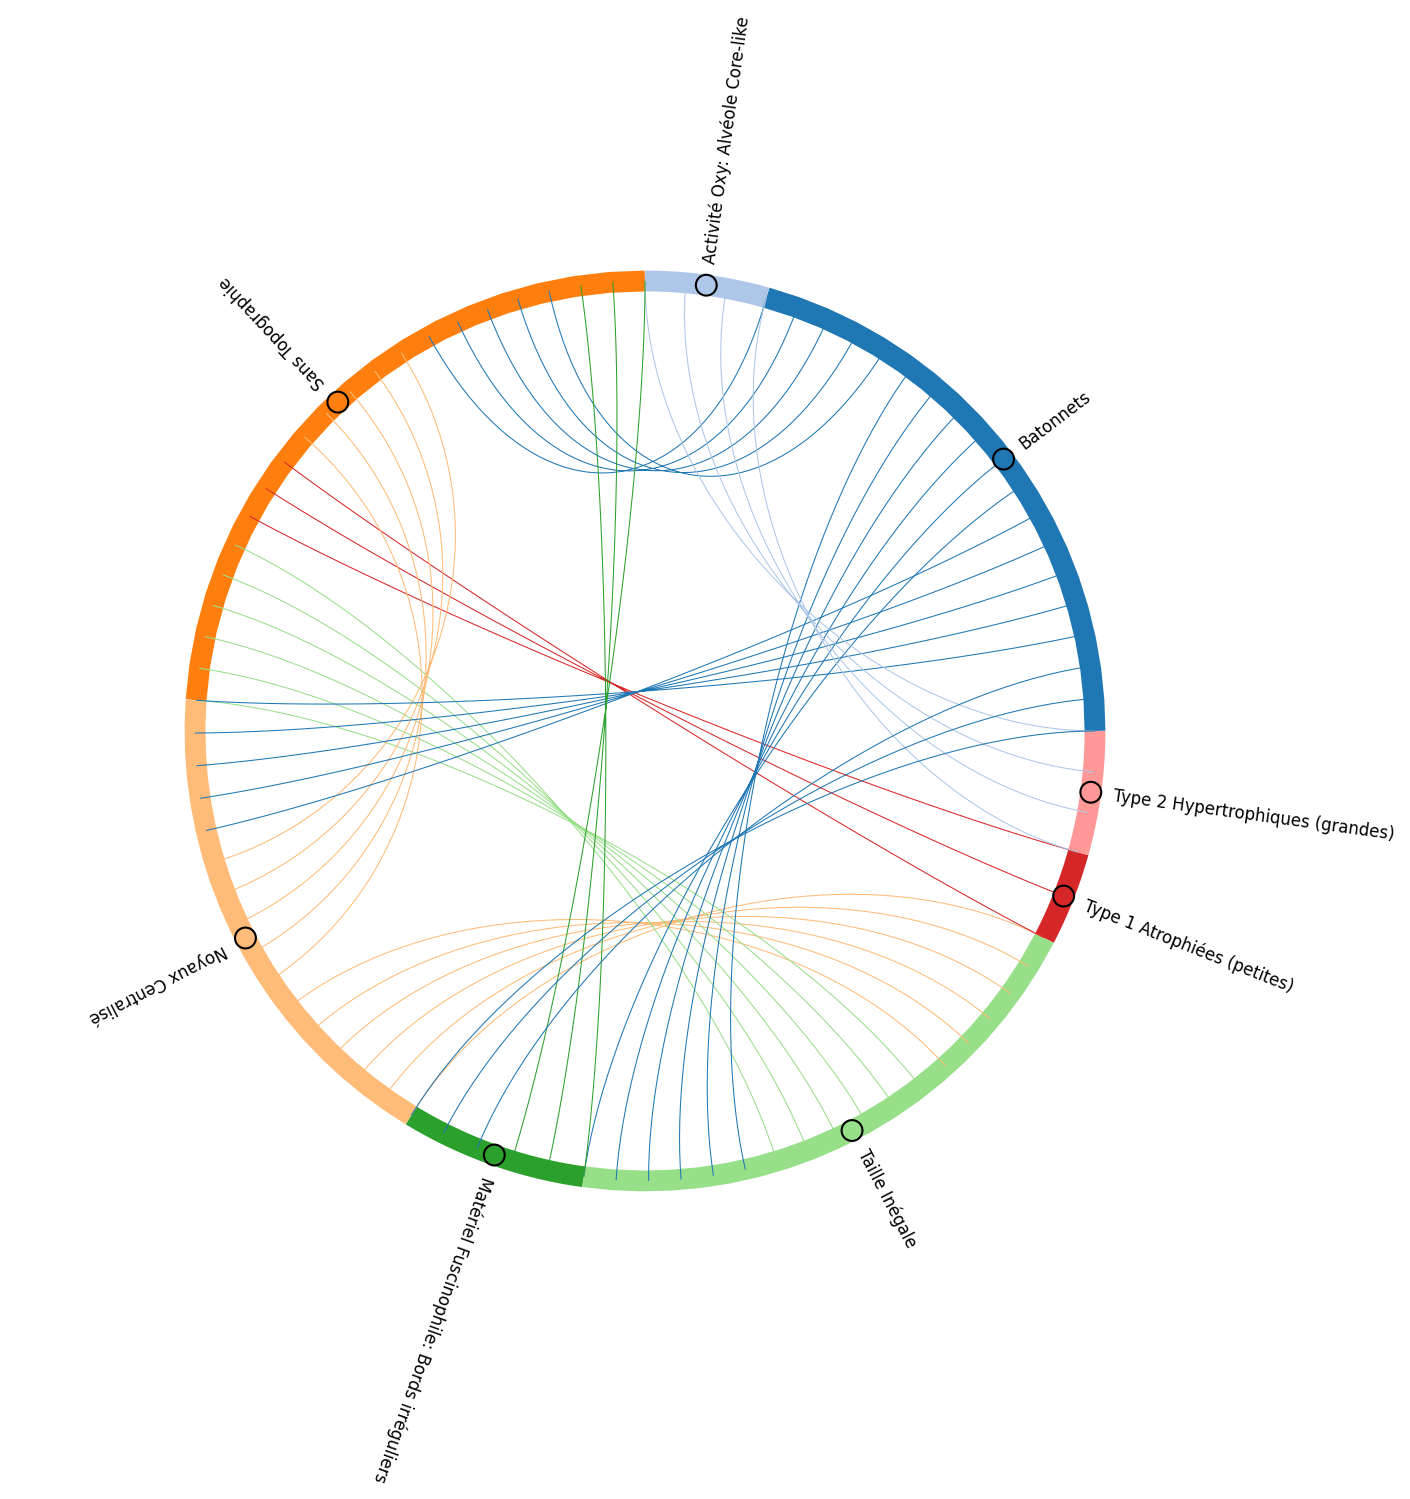
\includegraphics[width=1\textwidth]{figures/chord_plot.png}
  \caption[Diagramme de cordes des règles issues de l'entrainement de ExSTraCS]{\textbf{Diagramme de cordes des règles issues de l'entraînement de ExSTraCS}. Un lien entre deux termes indique que les deux termes apparaissent de manière commune dans une règle créée par le modèle. Plusieurs liens entre deux termes indiquent que ces liens apparaissent de manière commune dans plusieurs règles distinctes.}
  \label{fig:chords}
\end{figure}
La seconde approche a permis de générer le réseau représenté dans la figure \ref{fig:network}. Cette figure est disponible de manière interactive à l'adresse \url{https://lbgi.fr/~meyer/myomap.html} et dans l'archive Zenodo. On observe sur cette représentation que chaque diagnostic est lié à des termes exclusifs tel que la présence de nécrose et d'une augmentation du collagène endosymial pour les myopathies à némaline ou un trouve de l'activité phospholipases pour les myopathies à cores. On observe aussi que trois termes sont utilisés par les modèles pour discriminer entre les sous-types de myopathies en fonction de leur état. Par exemple, le terme "type 2 hypertrophiques" est lié de façon positive aux myopathies à cores et négativement aux myopathies à némaline et centronucléaires. À l'inverse, le terme bâtonnet est lié positivement aux myopathies à némaline, négativement aux myopathies à cores et de façon mixtes (jaune) aux myopathies centronucléaires. Enfin, on observe que cette visualisation permet de mettre en évidence de nouveaux termes présentés comment pertinents pour la classification des myopathies qui n'avaient pas été mis en évidence dans l'histogramme de l'importance des termes pour la classification présenté plus haut (fig. \ref{fig:feautre_importance}).
\begin{figure}[H]
  \centering
  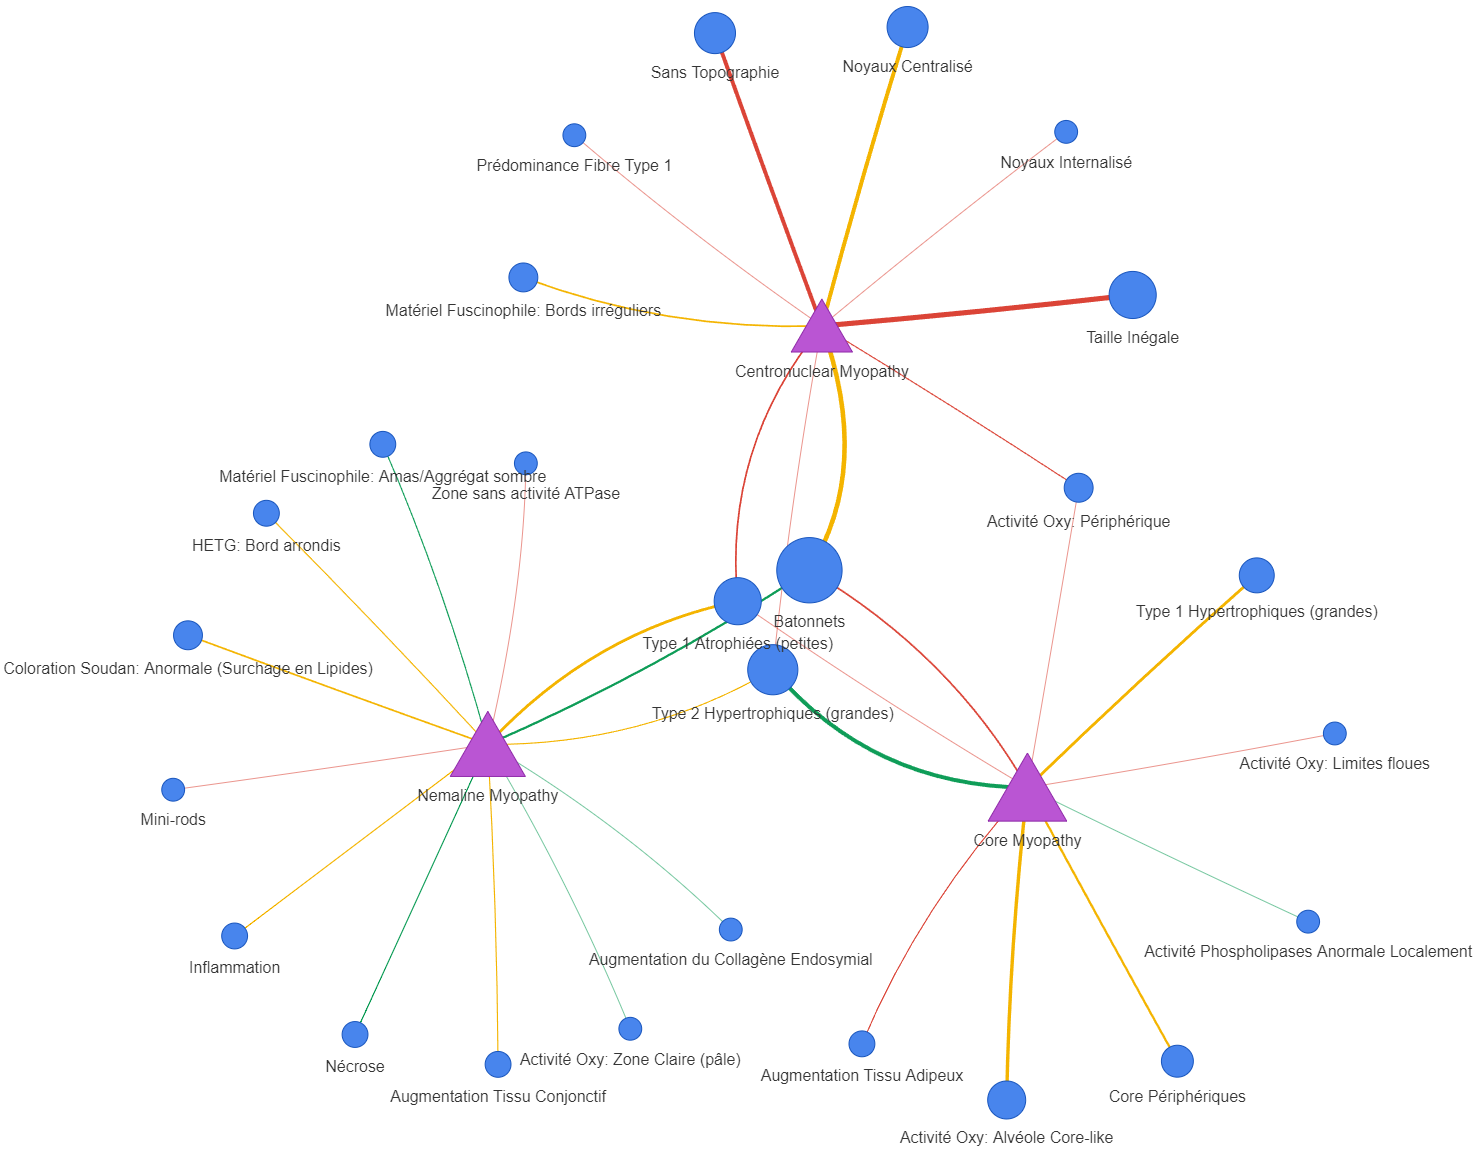
\includegraphics[width=1\textwidth]{figures/network_lcs.png}
  \caption[Représentation des règles issues de l'entraînement de ExSTraCS sous forme de réseau]{\textbf{Représentation des règles issues de l'entraînement de ExSTraCS sous forme de réseau}. Les triangles violets indiquent une classe (diagnostic de myopathie). Les nœuds bleus sont des termes du vocabulaire standard. Un lien vert indique un lien positif entre la classe et le terme, c'est-à-dire que le terme n'apparait que dans des règles liant sa présence au diagnostic. Un lien rouge indique que le terme n'apparait que dans des règles liant son absence au diagnostic. Un lien jaune indique des règles pouvant utiliser la présence ou l'absence du terme.}
  \label{fig:network}
\end{figure}
\section{Perspectives de développement}
En termes de développement futur, il est nécessaire d'agrandir le jeu de données utilisé pour comparer les algorithmes de classification. En effet, notre jeu de données de 89 rapports semble trop hétérogène et de trop petite taille pour déceler une différence significative de performances entre les algorithmes. De plus, il est nécessaire d'améliorer les approches de visualisation des règles de \gls{lcs}, car ces approches semblent être intéressantes pour visualiser graphiquement et rapidement le fonctionnement interne de notre système de classification explicable et pour identifier de nouveaux critères pertinents pour différencier les sous-types de myopathies congénitales.

Enfin, il pourrait être intéressant d'intégrer ce \textit{pipeline} d'entraînement et ces visualisations à \gls{impatient} pour entraîner automatiquement un modèle de classification explicable à base de règles et performant lors de l'entrée de nouveaux patients. De plus, l'intégration de ce modèle dans le formulaire d'ajout de nouveaux rapports dans la base de données pourrait permettre de réaliser de l'aide au diagnostic en suggérant automatiquement des diagnostics probablement et en mettant en évidence les règles à l'origine de cette classification.